\chapter{Project Management}


\section{Planning}\label{sec:planning}

\begin{tabular}{ l l l }
    \hline
    \bold{\textnumero} & \bold{Milestone}                       & \bold{Date of Achieval} \\ \hline
    MS\_1              & Cultivation of Bacteria                & 09.11.2023              \\
    MS\_2              & Extraction of LanM                     & 07.12.2023              \\
    MS\_3              & Detection of LanM                      & obsolete                \\
    MS\_4              & Binding of LanM to Rare Earth Elements & 29.02.2024              \\
    MS\_5              & Separation of Rare Earths from LanM    & n/d                     \\
    \hline
\end{tabular}


\section{Evaluation\authorA{}}

\begin{figure}[H]
    \centering
    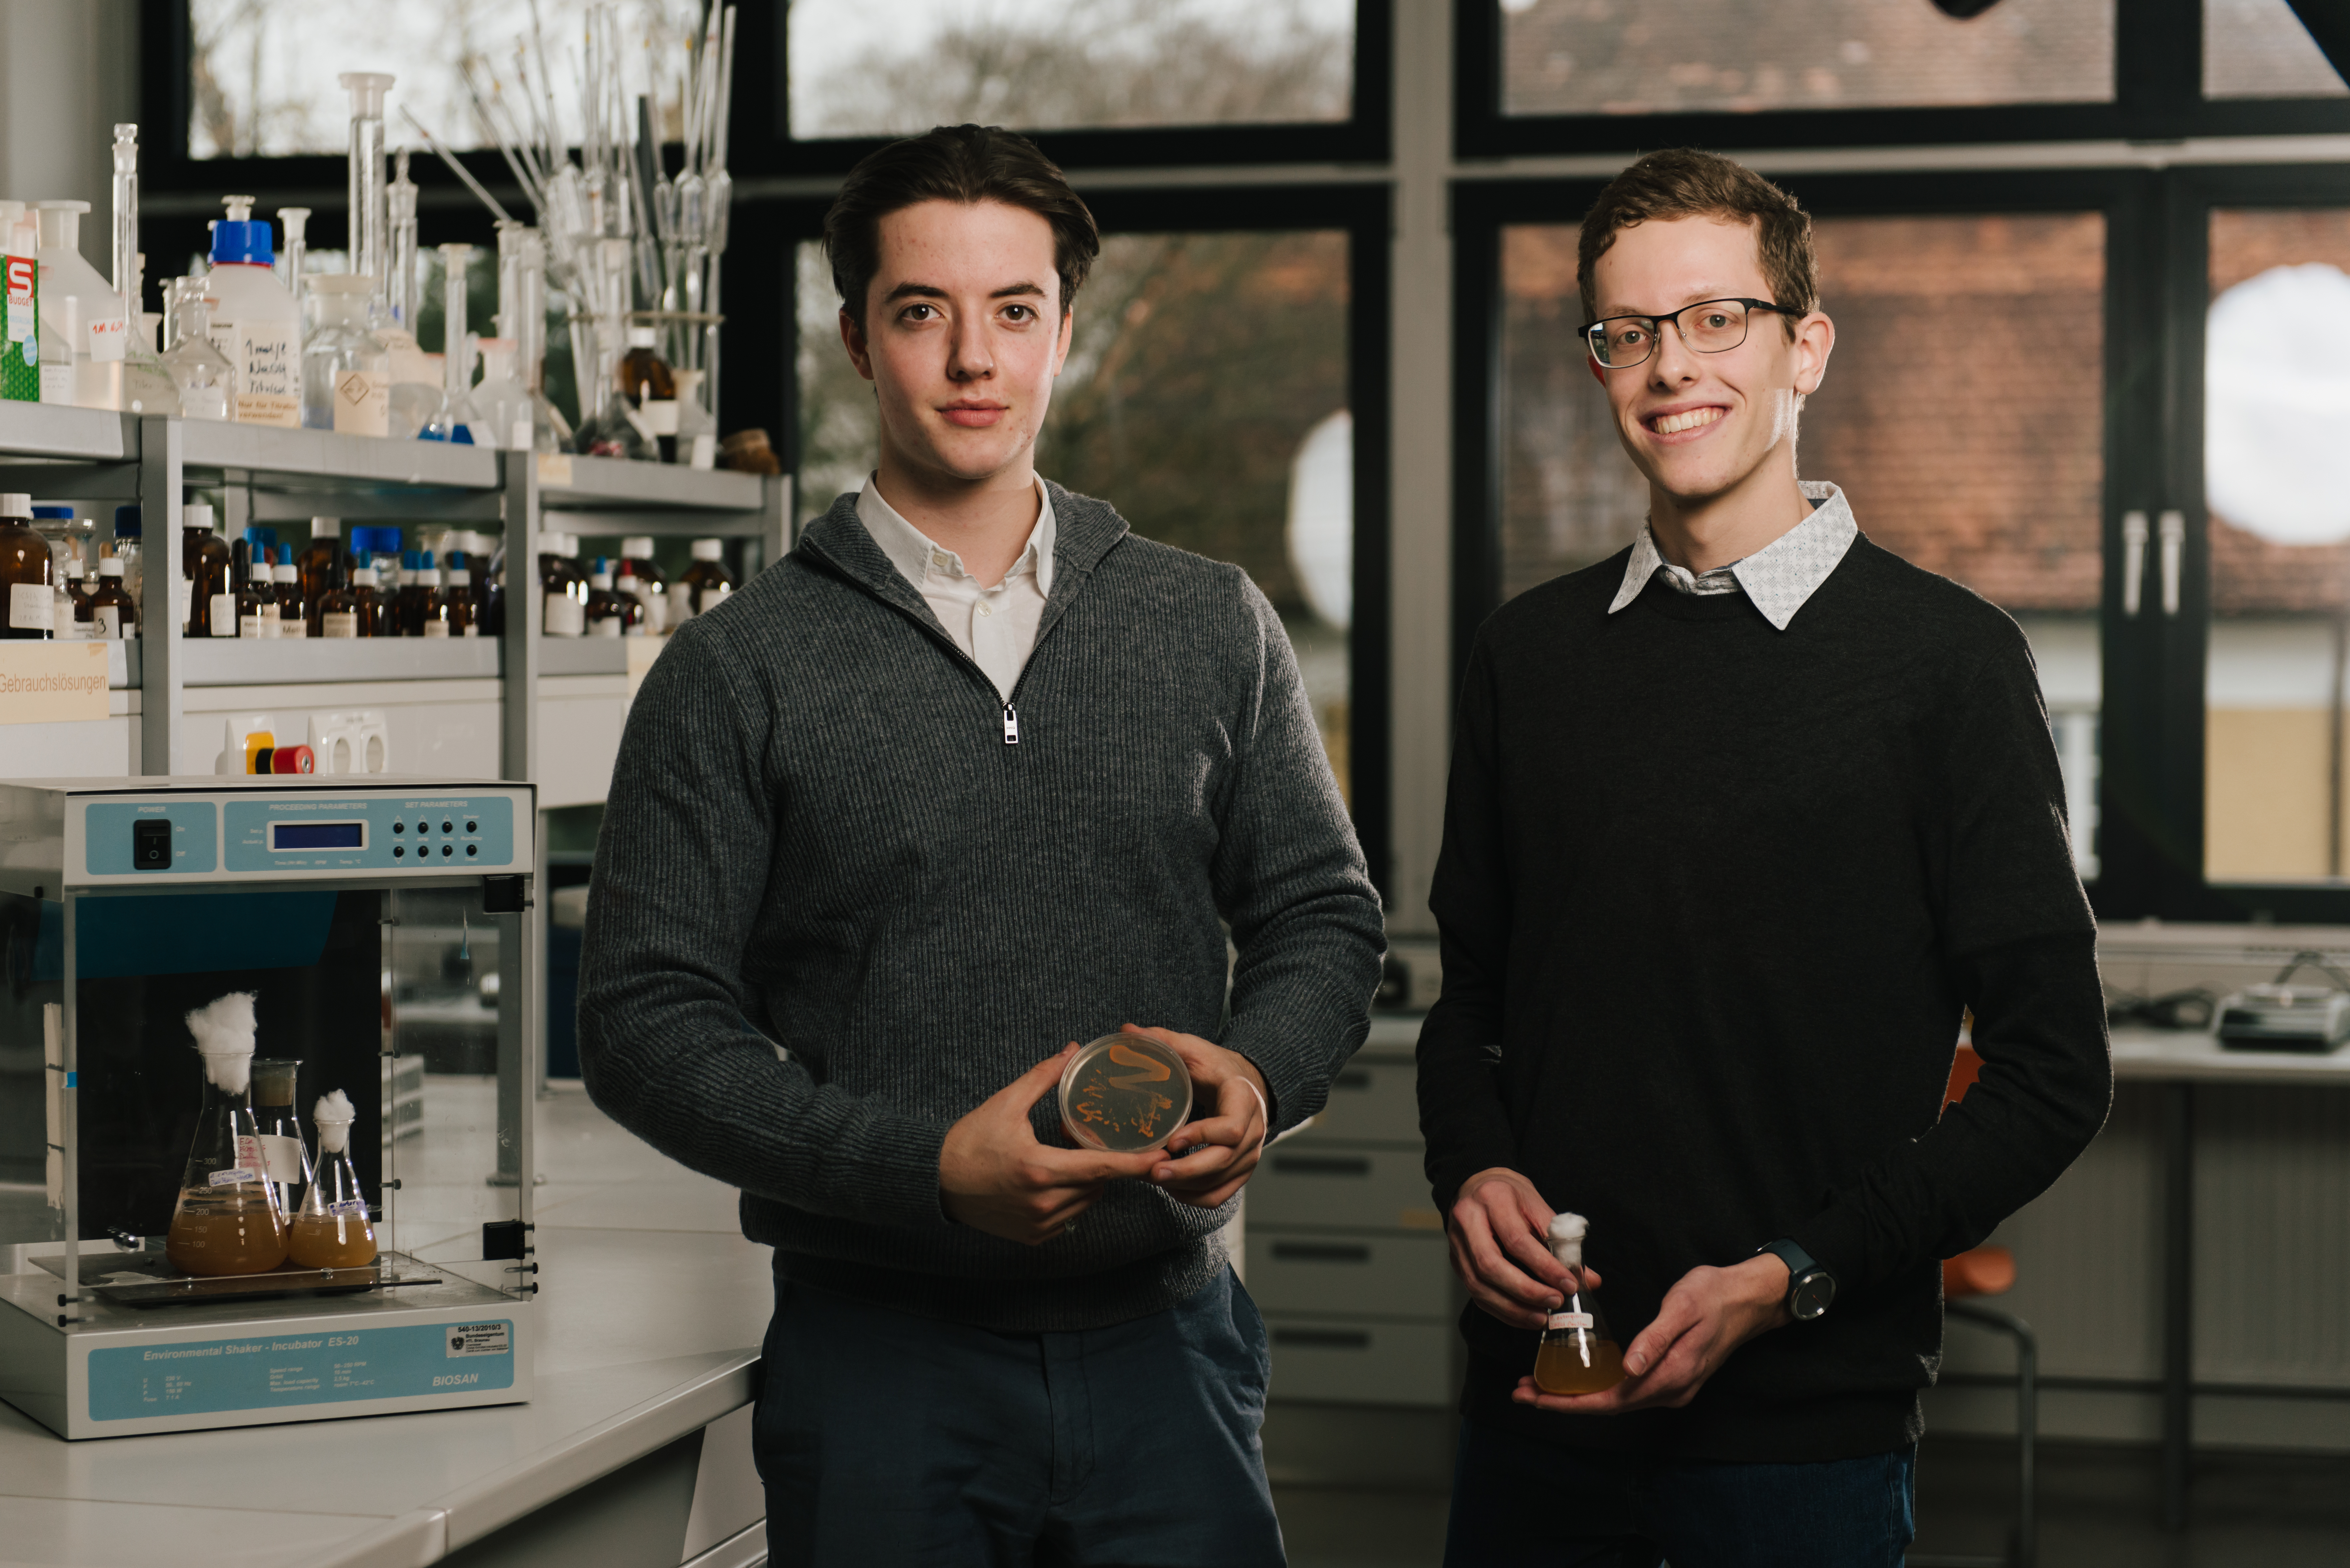
\includegraphics[width=0.8\textwidth]{./media/images/teamfoto}
    \caption{The project team}
    \label{fig:teamphoto}
\end{figure}

When we started to conduct some research for the project in the summer break, we also began simultaneously to plan the work with agile project management methods.
As it turned out, doing the project management this way was really helpful.
During our work, we encountered a lot of obstacles which we had not thought of before, which resulted in a slower progress than we had previously expected.

Another problem that we encountered was that we simply could not do our project the way we had planned at the beginning.
Due to limited financial and material resources, we could not carry out our planned work.
A lot of methods we tried out did not produce the expected or reliable results.
When we ran into these problems, we had to change how we want to achieve our planned goals.
This also meant that one of our planned milestones (MS\_3 Detection of LanM, see section~\ref{sec:planning}) is completely obsolete, because this step is simply not necessary anymore.

Our new approach requires less expensive resources and is simpler to carry out.
Overall, this made our project better, and it did not change our main goal.
The transformation from our first approach to the other would not have been possible if we had not used agile project management methods.



\newpage


\section{Timesheet}

\subsection{Tobias Daxecker}


\begin{tabularx}{\textwidth}{l p{1cm} l p{1cm} X}

    Braunau/Inn, \todayshort & & Tobias Daxecker & & \hrulefill                       \\
    \emph{Ort, Datum}        & &                 & & \emph{Unterschrift} \vspace{2cm} \\

\end{tabularx}

\subsection{Mathias Standhartinger}

\begin{tabularx}{\textwidth}{l p{1cm} l p{1cm} X}

    Braunau/Inn, \todayshort & & Mathias Standhartinger & & \hrulefill                       \\
    \emph{Ort, Datum}        & &                        & & \emph{Unterschrift} \vspace{2cm} \\

\end{tabularx}

